% Teilauswertung 4

\section{Lock-In Verstärker}
\label{sec:lockin}

\paragraph{a)}\textbf{Lock-In Verstärker als Filter}

Im folgenden Teil der Lock-In Verstärker als Filter verwenden und die Ausgangsmesswerte der Sinus, Rechteck und Dreieckschwingung interpretieren.

Die Messungen haben folgende Tabelle ergeben:
\begin{center}
    \begin{tabular}{l | c c c c c c c}
        f/kHz               & 1 & 3 & 5 & 7 & 9 & 11 & 13 \\
        \hline
        $U_{eff,Sinus}$/V     & 0,7072 & 0,0000 & 0,0000 & 0,0000 & 0,0000 & 0,0000 & 0,0000 \\
        $U_{eff,Rechteck}$/V  & 0,9003 & 0,3000 & 0,1800 & 0,1285 & 0,1000 & 0,0817 & 0,0692 \\
        $U_{eff,Dreieck}$/V   & 0,5733 & 0,0636 & 0,0229 & 0,0117 & 0,0070 & 0,0047 & 0,0034 \\
    \end{tabular}
    \captionof{table}{Messung Lock-In Verstärker als Filter bei unterschiedlichen Signalen}
    \label{tab:lockinFilter}
\end{center}
Wie in Tabelle \ref{tab:lockinFilter} schon angedeutet, handelt es sich bei den gemessenen Spannungswerte um die Effektivspannungswerte der jeweiligen Schwingung. Wie schon in Kapitel \ref{sec:mittelungAndTrafo}a) kann man die Effektivspannungswerte in die Werte der Fourierentwicklungskoeffizienten umrechnen, indem man die Messwerte mit dem Faktor $\sqrt{2}$ multipliziert. Zum Vergleich mit der Theorie werden die errechneten Werte aus Tabelle \ref{tab:fourierkoeff} verwendet und es werden wieder nur Rechteck- und Dreieckschwingung betrachtet. Weiterhin wird erneut die betragsmässige Differenz wie in Kapitel \ref{sec:fourierseries}a) berechnet. Damit erhält man:
\begin{center}
    \begin{tabular}{c | c c r | c c r}
        {} & \multicolumn{3}{c|}{\textbf{Rechteck}} & \multicolumn{3}{c}{\textbf{Dreieck}}\\
        $f$/kHz & $U_{Mess}$/V & $U_{Theo}$/V & $\Delta U$/$\mu$V & $U_{Mess}$/V & $U_{Theo}$/V & $\Delta U$/$\mu$V\\
        \hline
         1  & 1.273216 &  1.273240 &   23.07 &   0.810769 &   0.810569 &  199.17 \\
         3  & 0.424264 &  0.424413 &  149.11 &   0.089944 &   0.090063 &  119.29 \\
         5  & 0.254558 &  0.254648 &   89.47 &   0.032385 &   0.032423 &   37.29 \\
         7  & 0.181726 &  0.181891 &  164.92 &   0.016546 &   0.016542 &    4.06 \\
         9  & 0.141421 &  0.141471 &   49.70 &   0.009899 &   0.010007 &  107.54 \\
        11  & 0.115541 &  0.115749 &  207.80 &   0.006647 &   0.006699 &   52.12 \\
        13  & 0.097864 &  0.097942 &   77.92 &   0.004808 &   0.004796 &   12.06 \\
    \end{tabular}
    \captionof{table}{Vergleich Theorie und Praxis bei der Messung mit Lock-In Verstärker}
    \label{tab:lockinFourierkoeff}
\end{center} 
In Tabelle \ref{tab:lockinFourierkoeff} sieht man ganz deutlich wie präzise die Messung mit einem Lock-In Verstärkers ist. In der Berechnung hat man dabei bewusst auf die Fehlerrechnung verzichtet, da die Fehler nur in der Größenordnung von $\pm 0,0001$\,V liegen. Im Vergleich zu Tabelle \ref{tab:fourierkoeff} hat der Lock-In Verstärker aber eine deutlich höhere Präzession der Messung, da vor allem bei Frequenzen von 1\,kHz eine geringere Abweichung zu verzeichnen ist. Dies der Sachverhalt wurde im Verglaich mit den Ergebnis aus Kapitel \ref{sec:fourierseries}a) in Abbildung \ref{image:resiVergleich} dargestellt.
\begin{center}
    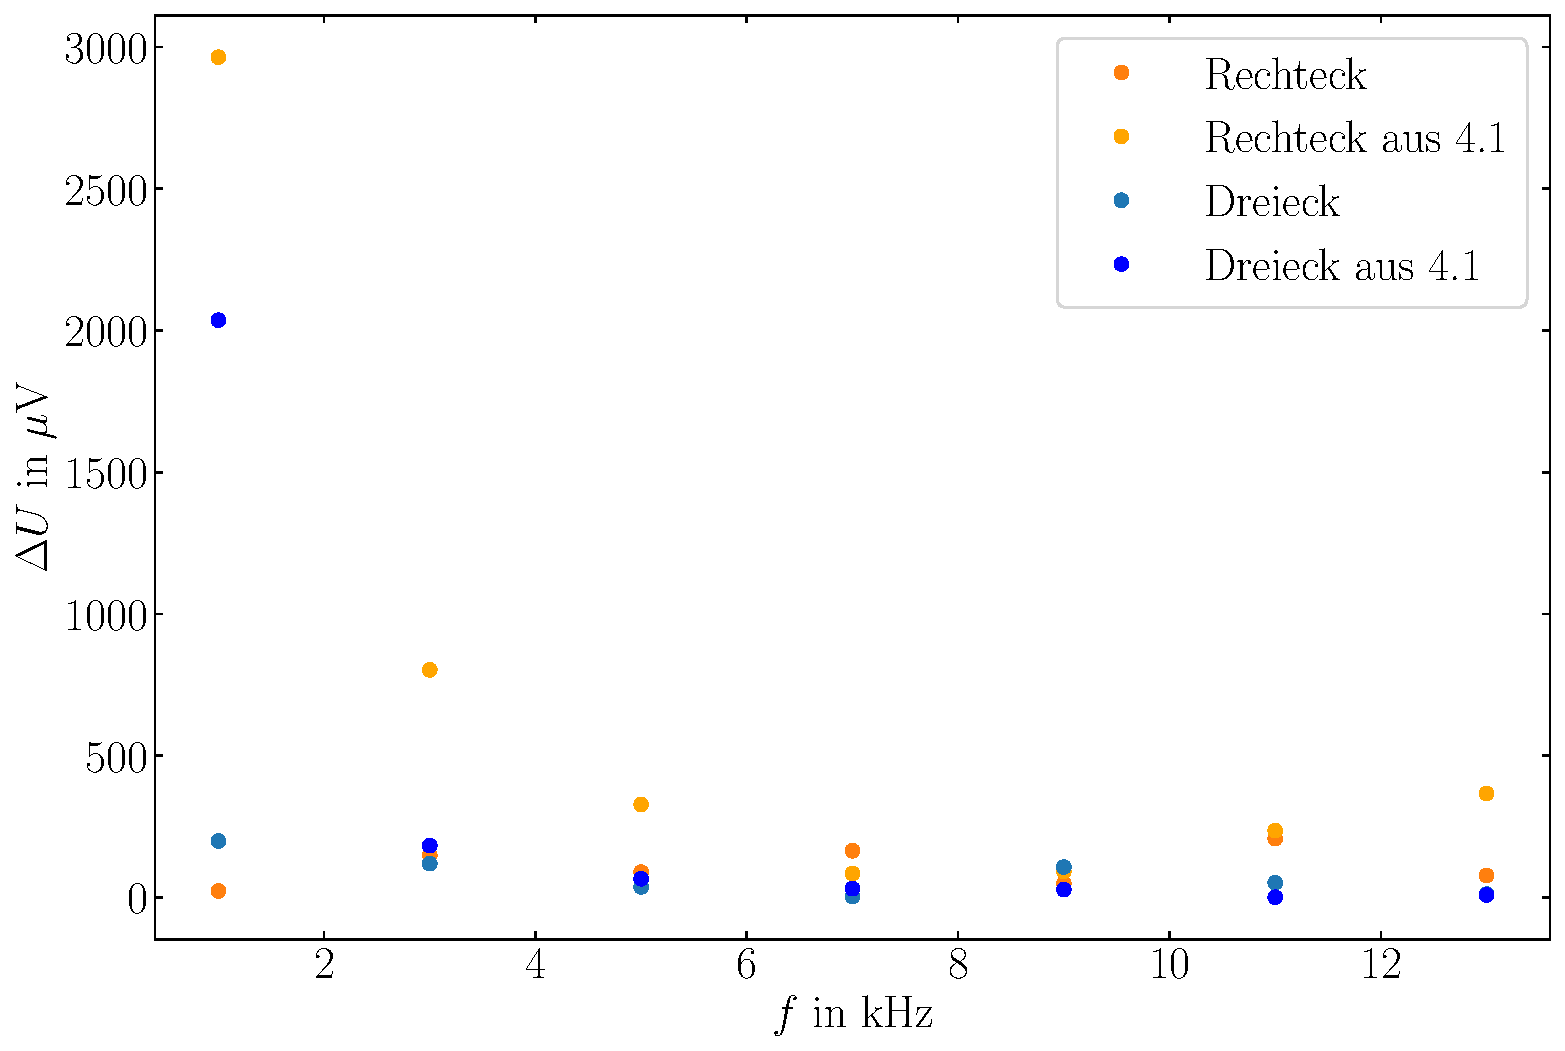
\includegraphics[scale=0.5]{Manuel/44/ResiduumVergleich.pdf}
    \captionof{figure}{Vergleich der betragsmässigen Differenz zwischen Ergebnis aus Kapitel 4.4a) und Kapitel 4.1a)}
    \label{image:resiVergleich}
\end{center} 

\newpage
\paragraph{b)}\textbf{Bandbreite des Lock-In Verstärkers}

Als Nächstes wird die Zeitkonstante $\tau$ und die Ordnung $n$ des Filters des Lock-In Verstärkers bestimmt. Dafür wurde an dem Lock-In Verstärker eine Sinusschwingung mit einer Frequenz von 1\,kHz und eine Amplitude von 100\,mV angelegt. Am Lock-In Verstärker wurde die Flankensteilheit $\Delta$ des eingebauten Tiefpassfilters von 6\,dB auf 18\,dB verändert und eine Zeitkonstante $\tau$ von 30\,ms eingestellt. Um die Zeitkonstante und Ordnung zu bestimmen wird eine Kurve durch die aufgenommene Messreihe gefittet. Die Form der Kurve wurde im Praktikum zur Verfügung besprochen und ist speziell für den Lock-In Verstärker SR830 DSP. Die Kurve hat dann die Gleichung:
\begin{gather}
    A_{\tau,n}(f) = \left[1 + (2\pi\tau(f-f_0))^2\right]^{-\frac{n}{2}}
\end{gather}
Diese Gleichung beschreibt hierbei die Filterantwort des Lock-In Verstärkers, wobei \newline $n$ die Ordnung, $\tau$ die Zeitkonstante des Filters und $A$ die normierte Amplitude ist. Die Frequenz $f_0$ ist die eingestellte Frequenz der Sinusschwingung und liegt bei 1kHz. Die Normierung erfolgt über den maximalen Wert der Effektivspannung, welcher bei den Frequenz $f_0$ liegt. Durch die Normierung muss die Umwandlung von Effektivspannung in tatsächliche Spannung nicht berücksichtigt werden. Es wurde wieder auf eine Fehlerrechnung verzichtet, da die Fehler der Messwerte zu klein sind. Der Fit liefert dann folgende Parameter:
\begin{center}
    \begin{tabular}{c | c c}
        $\Delta$/dB & $\tau$/ms & $n$\\
        \hline
        6  & 27,35 & 1,06 \\
        18 & 30,16 & 3,00 \\
    \end{tabular}
    \captionof{table}{Ergebnis gefittete Parameter für $\tau$ und $n$}
    \label{tab:fitPara}
\end{center}
In Abbildung \ref{image:6dB} und \ref{image:18dB} ist jeweils der Fit für die jeweilige Messreihe dargestellt. Der Vergleich der gefitteten Werte der Zeitkonstante $\tau$ mit dem tatsächlichen eingestellten Wert von 30ms zeigt, dass die Messung des Lock-In Verstärkers eine genaue Bestimmung der Zeitkonstante $\tau$ zulässt. Ein guter Indikator ist hierbei die Ordnung $n$, da die tatsächliche Zeitkonstante $\tau$ dann erzielt wurden als $n$ ganzzahlig war.

Auch ist zu erkennen, dass durch eine Verdreifachung der Flankensteilheit $\Delta$ sich die Ordnung $n$ des Filters verdreifacht. Dies zeigt auch Abbildung \ref{image:All}, in der die gefittete Kurve für $\Delta=18$\,dB viel schmäler ist als die gefittete Kurve für $\Delta=6$\,dB.
\newpage
\begin{center}
    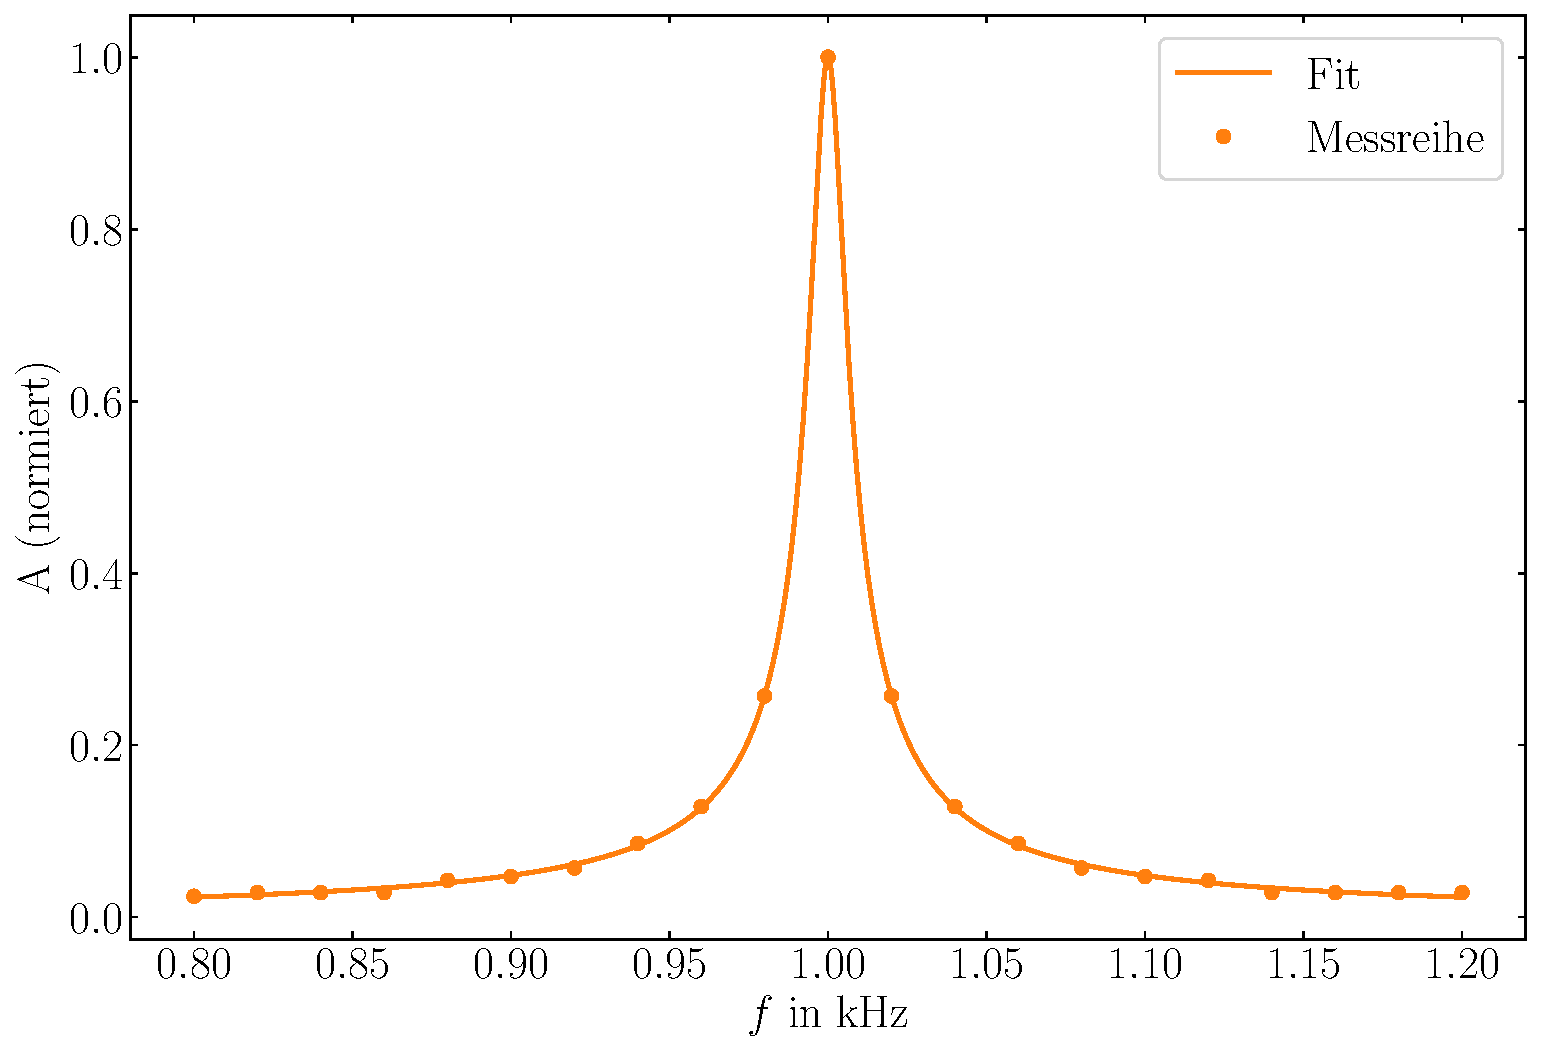
\includegraphics[scale = 0.5]{Manuel/44/6dB.pdf}
    \captionof{figure}{Fit für die Messung mit $\Delta$=6\,dB}
    \label{image:6dB}
    \vspace{1cm}
    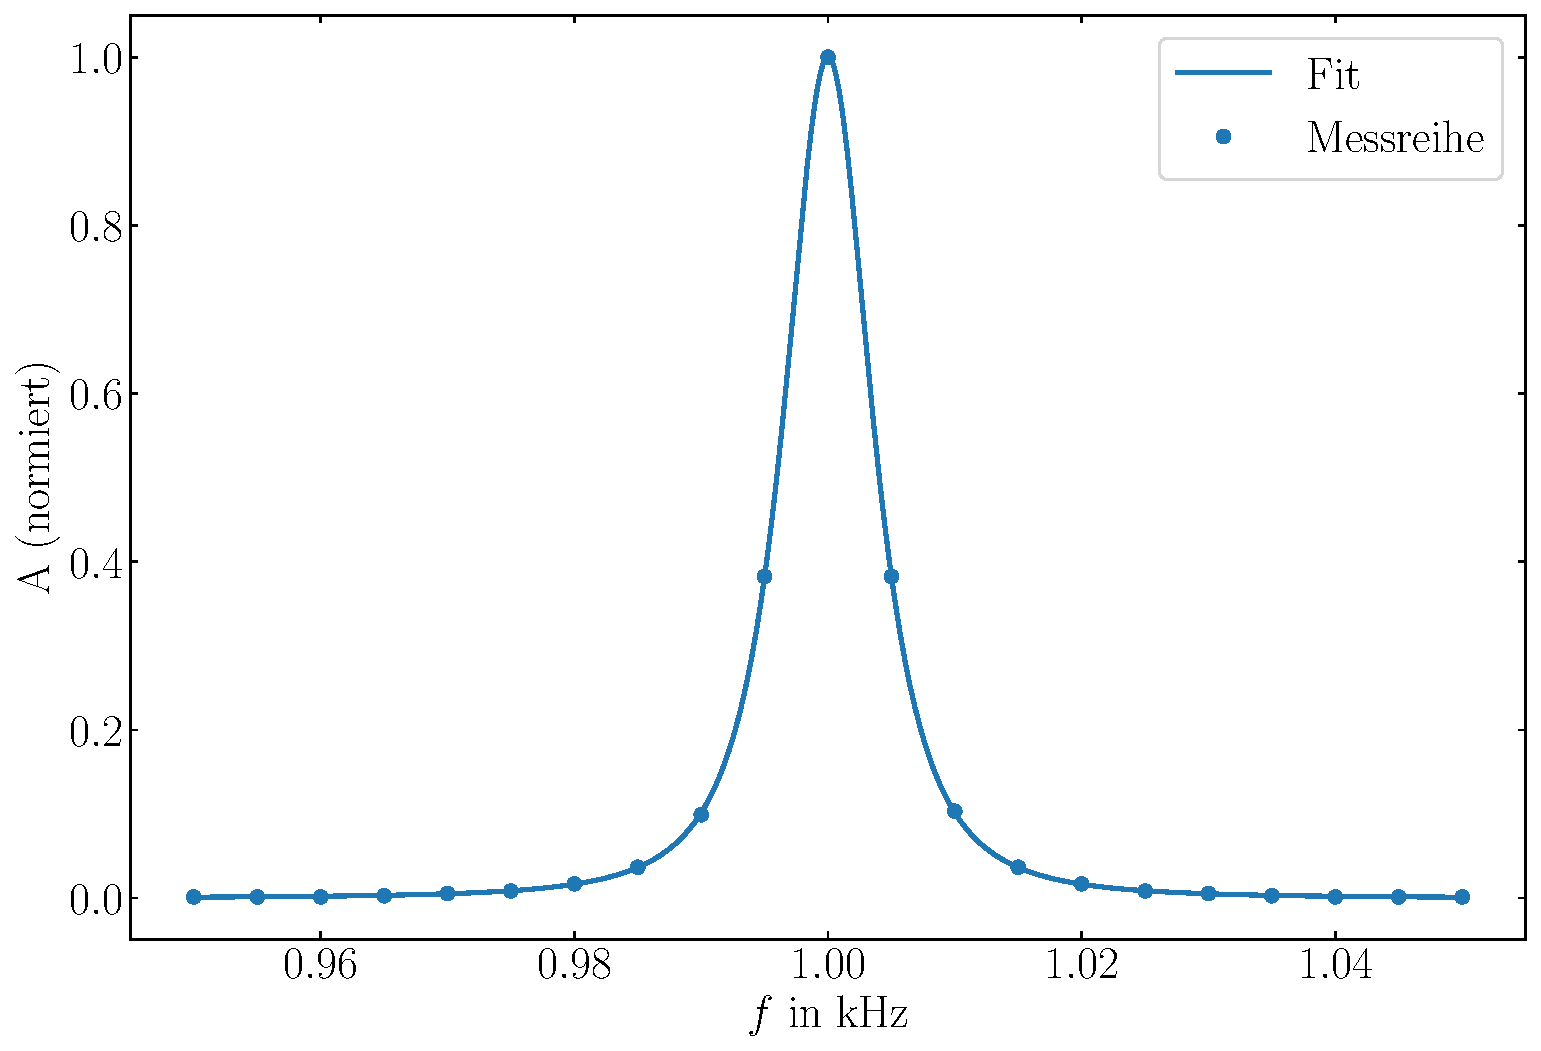
\includegraphics[scale = 0.5]{Manuel/44/18dB.pdf}
    \captionof{figure}{Fit für die Messung mit $\Delta$=18\,dB}
    \label{image:18dB}
    \vspace{1cm}
    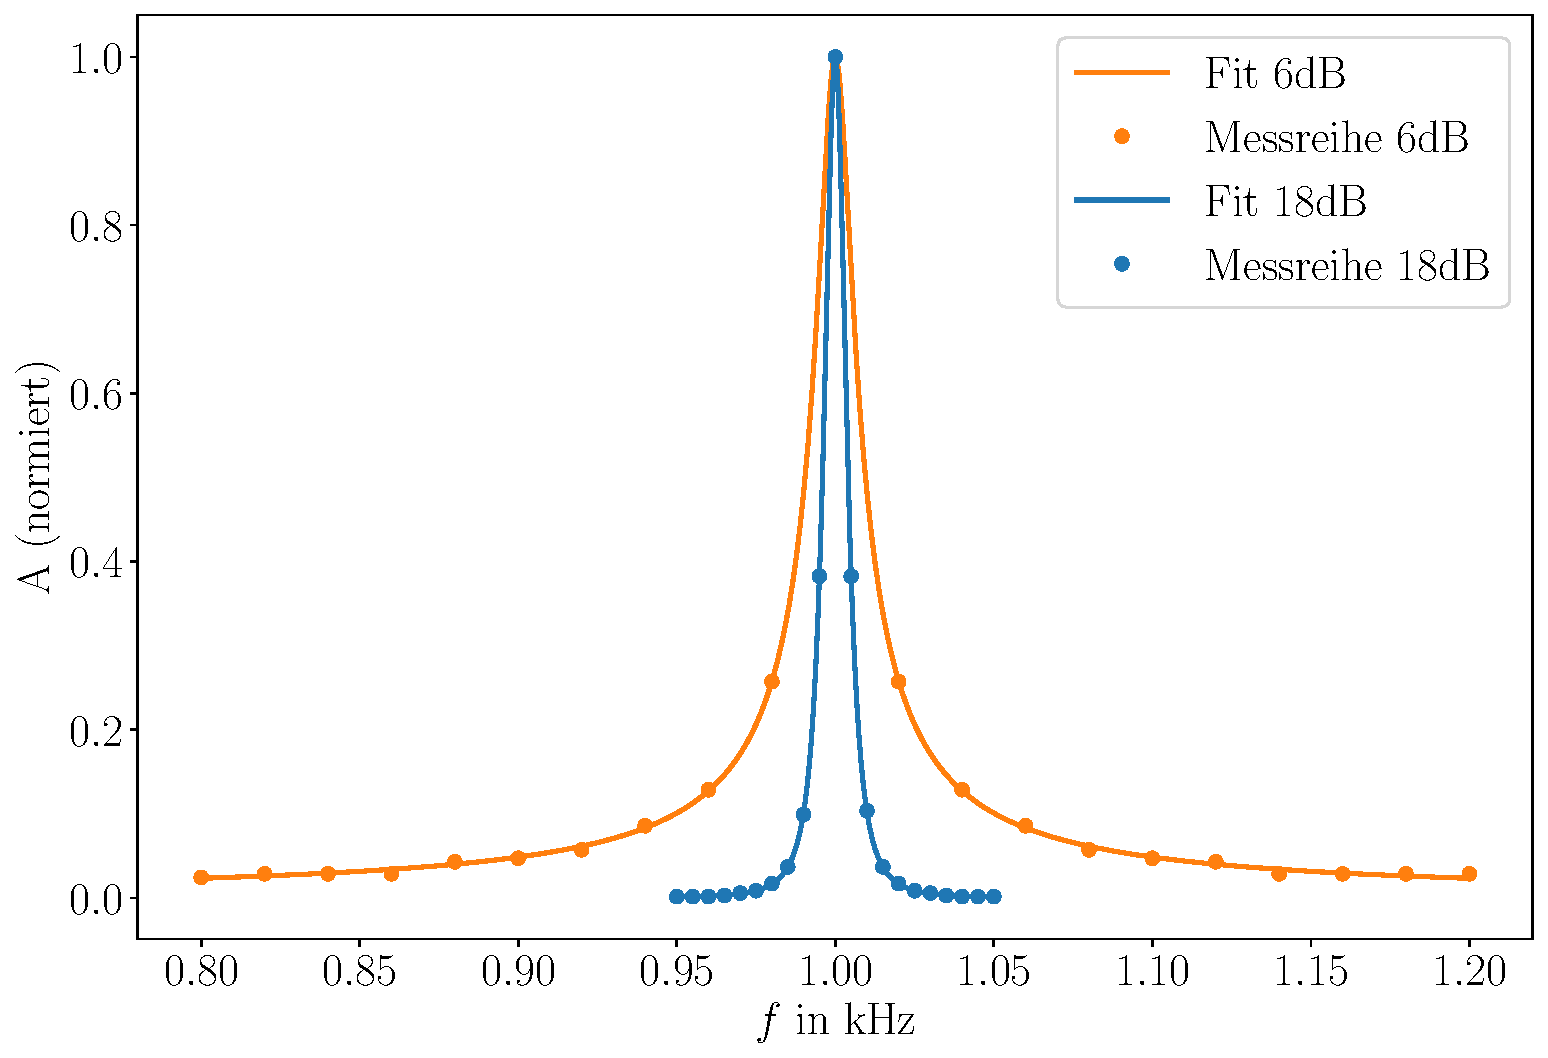
\includegraphics[scale = 0.5]{Manuel/44/All.pdf}
    \captionof{figure}{Vergleich beider Messreihen mit Fit}
    \label{image:All}
\end{center}

\paragraph{c)}\textbf{Lock-In in Praxis}

Im letzten Abschnitt wird noch die Verwendung eines Lock-In Verstärkers in der Praxis besprochen. Dazu stand eine Leuchtdiode und eine Photodiode in einer Box mit Deckel zur Verfügung. Die Signale von Leuchtdiode und Photodiode wurden dann auf dem Oszilloskop betrachtet. Man konnte beobachten, dass bei offenen Deckel große Schwankungen am Oszilloskop entstanden. Dies kann damit erklärt werden, das die Photodiode neben dem Signal der Leuchtdiode auch das Licht der Beleuchtung des Raums registriert hat, welches mit 50\,Hz flackert. Wurde der Deckel geschlossen, ließen die Schwankung nach und die Photodiode detektierte nur noch das Signal der Leuchtdiode, welches trotzdem sehr verrauscht war (zu sehen in Abb. \ref{image:oszi}). 

Die Änderung der Zeitkonstante $\tau$ und Flankensteilheit $\Delta$ am Lock-In Verstärker ergaben eine Veränderung der Auflösung des Lock-In Verstärkers. Dabei war die Auflösung am höchsten, wenn auch die Zeitkonstante und Flankensteilheit am höchsten waren.

%Die Bandbreite des Lock in Verstärkers lässt sich über die Grenzfrequenz $f_g$ bestimmen. Diese ist proportional zu $\frac{1}{\tau}$. In der Messung ist $\tau = 1$\,s (aus Abb. \ref{image:lockIn}), womit $f_g\approx 1$\,Hz ist, was der Bandbreite des Lock-In Verstärkers entspricht. Um diese Größe in dB umzurechnen, wird eine Referenzfrequenz benötigt, welche nicht beim Versuch aufgezeichnet wurde.

Die Detektionsbandbreite $B$ des Lock-In Verstärkers lässt sich wie folgt berechnen:
\begin{gather}
    B = 20\log_{10}\left(\frac{U_{min}}{U_{max}}\right)
\end{gather}
Bei dem verwendeten Loch-In Verstärker ist die maximale Spannung $U_{max}=$ 1\,V, was durch Bauart des Gerätes bedingt ist, und die minimal Spannung $U_{min} =$ 255\,nV. Damit ergibt sich eine Detektionsbreite $B =$ -132\,dB.